Der Begriff CRUD steht für Create, Read, Update und Delete. Dies sind vier grundlegende Operationen in der Datenverarbeitung. Oft bilden diese Operationen die grundlegende Schnittstelle zwischen Andwendungen und Datenbanken.

\begin{figure}[h!]
    \centering
    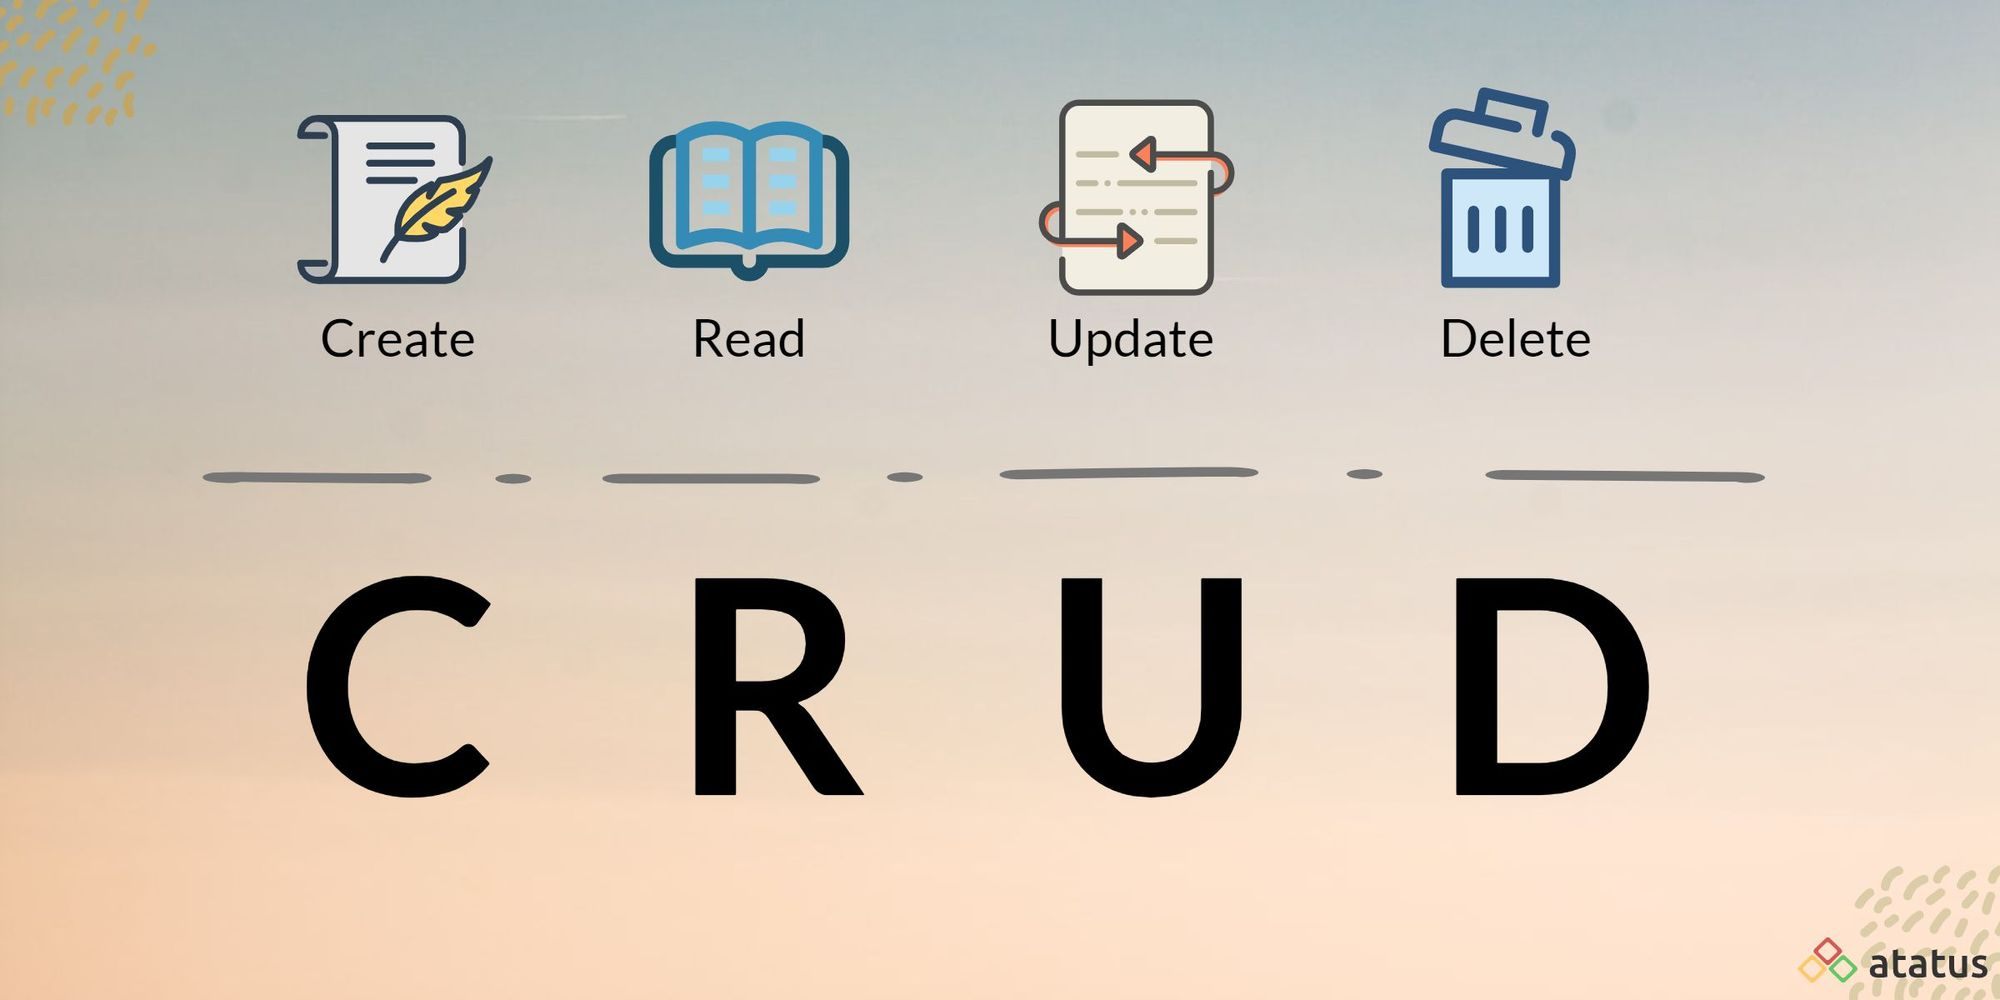
\includegraphics[width=0.6\textwidth]{pics/CRUD.jpeg}
    \caption{CRUD Operations}
    \label{fig:enter-label}
\end{figure}


 \subsection{Create}

 Bei der Create Operation geht es darum, neue Daten in die Datenbank zu persistieren. Dies kann zum Beispiel sein ein Benutzerprofil anzulegen oder einen neuen Plan hinzuzufügen. 


 \subsection{Read}

 Die Read-Operation ergmöglicht es, vorhanende Daten aus der Datenbank auszulesen. Dies erfolgt in der Form von Abfragen um Datensätze nach bestimmten Kritierien zu filtern oder auch gegebenenfalls alle Datensätze abzurufen.


\subsection{Update}

Die Update-Operation wird verwendet, um bereits bestehende Datensätze in der Datenbank zu verändern. Das können beispielsweise Anpassungen von Adressen in einer Kundendatenbank oder Preisänderungen in einer Produktdatenbank sein. Ähnlich wie bei READ-Operationen können UPDATE-Operationen, abhängig von den ausgewählten Kriterien, auf sämtliche Datensätze oder nur auf ausgewählte beschränkt werden.

Manche Big-Data-Systeme verzichten gänzlich auf die Integration der UPDATE-Operation und ermöglichen stattdessen ausschließlich eine CREATE-Operation in Verbindung mit einem Zeitstempel. Dabei wird bei jeder Aktualisierung eine neue Version der Zeile hinzugefügt.


\subsection{Delete}


Die DELETE-Operation erlaubt es dem Nutzer, Datensätze aus der Datenbank zu löschen. Bei einem endgültigen Löschen wird der Datensatz vollständig entfernt, während er beim vorläufigen Löschen markiert, aber an seinem aktuellen Ort belassen wird.



Im Falle dieser Diplomarbeit wurden auschließlich READ und UPDATE-Operations verwendet. Die Syntax um ein Projekt zu löschen sieht wie folgt aus.

\begin{lstlisting}
    const project = await Projects.findById(req.params.id)

  try {
    project.trashed = req.body.value.new
    project.trashedDate = new Date()

    await project.save()

    res.json({ success: true })
  } catch (e) {
    next(e)
  }
\end{lstlisting}

Zu Beginn wird die Suche nach dem Projekt anhand der ID durchgeführt. Anschließend wird in einem Try-Catch-Statement versucht, zwei Eigenschaften zu modifizieren. Zum einen wird das Attribut "project.trashed" angepasst, das vom Datentyp Boolean ist und daher entweder den Wert "true" oder "false" annehmen kann. Zusätzlich wird das Attribut "project.trashedDate" gesetzt, das vom Datentyp "Date" ist, um den exakten Zeitstempel zu dokumentieren, wann die Änderung am Projekt vorgenommen wurde.

Im Anschluss wird das Projekt erneut gespeichert. Wenn sämtliche Operationen erfolgreich verlaufen, erfolgt über "res.json" eine Response, die einen Boolean zurückliefert welcher "true" zurückliefert.


Weiters wurden die Änderung des Speicherplatzes, sowie die Änderung des Abonnements nach dem selben Prinzip implementiert.

\cite{CRUD_Operations}